%!TEX program = xelatex
\documentclass[10pt, compress]{beamer}
\usetheme[titleprogressbar]{m}

\usepackage{booktabs}
\usepackage[scale=2]{ccicons}
\usepackage{minted}

\usepgfplotslibrary{dateplot}

\usemintedstyle{trac}

\setbeamertemplate{caption}[numbered]
\setbeamertemplate{theorems}[numbered]
\newtheorem{crl}{Corollary}[theorem]
\newtheorem*{solution*}{Solution}

\usepackage{algorithm}
\usepackage[noend]{algpseudocode}

\usepackage{version}
%\excludeversion{proof}
%\excludeversion{solution*}

\usepackage{mathtools}
\usepackage{multicol}
\usepackage{qtree}

\usepackage{tikz}

\makeatletter
\def\old@comma{,}
\catcode`\,=13
\def,{%
	\ifmmode%
	\old@comma\discretionary{}{}{}%
	\else%
	\old@comma%
	\fi%
}
\makeatother

\title{CSCI 3190 Tutorial of Week 03}
\subtitle{Relations}
\author{LI Haocheng}
\institute{Department of Computer Science and Engineering}

\begin{document}

\maketitle

\begin{frame}[fragile]
	\frametitle{Inverse Relation}
	\begin{columns}
		\begin{column}{.6\linewidth}
			Let $R$ be a relation from a set $A$ to a set $B$.
			\begin{definition}
				The \textbf{inverse relation} from $B$ to $A$, denoted by $R^{-1}$, is the set of ordered pairs $\{(b, a) \mid (a, b) \in R \}$.
			\end{definition}
			\begin{definition}
				The \textbf{complementary relation} $\bar{R}$ is the set of ordered pairs $\{(a, b) \mid (a, b) \notin R \}$.
			\end{definition}
		\end{column}
		\begin{column}{.4\linewidth}
			\begin{example}
				Let $R$ be the relation $R = \{(a, b) \mid a < b\}$ on the set of integers. Find \begin{enumerate}
					\onslide<1->\item $R^{-1}$ \onslide<2>$= \{(a, b) \mid a > b\}$
					\onslide<1->\item $\bar{R}$ \onslide<2>$= \{(a, b) \mid a \ge b\}$
				\end{enumerate}
			\end{example}
		\end{column}
	\end{columns}
\end{frame}

\begin{frame}[fragile]
	\frametitle{Division}
	\begin{columns}
		\onslide<1->\begin{column}{.5\linewidth}
			\begin{example}
				Let $R$ be the relation $R = \{(a, b) \mid a \text{ divides } b\}$ on the set of integers. Find \begin{enumerate}
					\onslide<1->\item $R^{-1}$ \onslide<2->$= \{(a, b) \mid b \text{ divides } a\}$
					\onslide<1->\item $\bar{R}$ \onslide<2->$= \{(a, b) \mid a \text{ doesn't divide } b\}$
				\end{enumerate}
			\end{example}
		\end{column}
		\onslide<1->\begin{column}{.5\linewidth}
			\begin{example}
				Let $R$ be the relation on the set of all districts in Hong Kong consisting of pairs $(a, b)$ where district $a$ borders district $b$. Find \begin{enumerate}
					\onslide<1->\item $R^{-1}$ \onslide<3>$= \{(a, b) \mid a \text{ borders } b\}$
					\onslide<1->\item $\bar{R}$ \onslide<3>$= \{(a, b) \mid a \text{ doesn't border } b\}$
				\end{enumerate}
			\end{example}
		\end{column}
	\end{columns}
\end{frame}

\begin{frame}[fragile]
	\frametitle{One-to-One Correspondence}
	\begin{example}
		Suppose that the function $f$ from $A$ to $B$ is a one-to- one correspondence. Let $R$ be the relation that equals the
		graph of $f$. That is, $R = \{(a, f(a)) \mid a \in A\}$. What is the inverse relation $R^{-1}$?
	\end{example}
	\onslide<2>\begin{solution*}
		The graph of $f^{-1}$.
	\end{solution*}
\end{frame}

\begin{frame}[fragile]
	\frametitle{Closures}
	\begin{columns}
		\begin{column}{.5\linewidth}
			\begin{definition}
				A \textbf{reflexive closure} of $R$\begin{enumerate}
					\item contains $R$,
					\item is reflexive,
					\item is contained within every reflexive relation that contains $R$.
				\end{enumerate}
			\end{definition}
			\begin{definition}
				A \textbf{diagonal relation} $\Delta$ on $A$ is $\{(a, a) \mid a \in A \}$.
			\end{definition}
		\end{column}
		\begin{column}{.5\linewidth}
			\begin{theorem}
				Given a relation $R$ on a set $A$, the reflexive closure of $R$ equals $R \cup \Delta$.
			\end{theorem}
			\onslide<2>\begin{proof}
				\begin{enumerate}
					\item $R \cup \Delta \supseteq R$.
					\item $R \cup \Delta \supseteq \Delta$.
					\item If there exists a reflexive set $S \supset \Delta$, $r \in R \cup \Delta$, $r \notin S$. Therefore $r \notin \Delta$, $r \in R$ so that $S \nsupseteq R$ which forms a contradictory.
				\end{enumerate}
			\end{proof}
		\end{column}
	\end{columns}
\end{frame}

\begin{frame}[fragile]
	\frametitle{Reflexive Closure}
	\onslide<1->\begin{example}
		What is the reflexive closure of the relation $R = \{(a, b) \mid a < b\}$ on the set of integers?
	\end{example}
	\onslide<2>\begin{solution*}
		\begin{align}
			\begin{aligned}
			& R \cup \Delta \\
			= & \{(a, b) \mid a < b \} \cup \{(a, a) \mid a \in \mathbb{Z}\} \\
			= & \{(a, b) \mid a \le b\}.
			\end{aligned}
		\end{align}
	\end{solution*}
\end{frame}

\begin{frame}[fragile]
	\frametitle{Symmetric Closure}
	\begin{columns}
		\begin{column}{.4\linewidth}
			\begin{definition}
				A \textbf{symmetric closure} of $R$\begin{enumerate}
					\item contains $R$,
					\item is symmetric,
					\item is contained within every reflexive relation that contains $R$.
				\end{enumerate}
			\end{definition}
		\end{column}
		\begin{column}{.6\linewidth}
			\begin{theorem}
				Given a relation $R$ on a set $A$, the reflexive closure of $R$ equals $R \cup R^{-1}$.
			\end{theorem}
			\onslide<2>\begin{proof}
				\begin{enumerate}
					\item $R \cup R^{-1} \supseteq R$.
					\item $(R \cup R^{-1})^{-1} = R^{-1} \cup {R^{-1}}^{-1} = R \cup R^{-1}$.
					\item If there exists a set $S \supseteq R$, $r \in R \cup R^{-1}$, $r \notin S$. Therefore $r \notin R$, $r \in R^{-1}$ so that $S \ne S^{-1}$ which forms a contradictory.
				\end{enumerate}
			\end{proof}
		\end{column}
	\end{columns}
\end{frame}

\begin{frame}[fragile]
	\frametitle{Example of Symmetric Closure}
	\begin{example}
		What is the symmetric closure of the relation $R =\{(a, b) \mid a > b\}$ on the set of positive integers?
	\end{example}
	\onslide<2>\begin{solution*}
		\begin{align}
		\begin{aligned}
		& R \cup R^{-1} \\
		= & \{(a, b) \mid a > b \} \cup \{(a, a) \mid a < b\} \\
		= & \{(a, b) \mid a \ne b\}.
		\end{aligned}
		\end{align}
	\end{solution*}
\end{frame}

\begin{frame}[fragile]
	\frametitle{Equivalence Relation}
	\begin{definition}
		A relation on a set $A$ is called an \textbf{equivalence relation} if it is reflexive, symmetric, and transitive.
	\end{definition}
	\begin{example}
		Let $R$ be the relation on the set of real numbers such that $(a, b) \in R$ if and only if $a - b$ is an integer. Is $R$ an equivalence relation?
	\end{example}
	\begin{solution*}
		Because $a - a = 0$ is an integer for all real numbers $a$, $\forall a \in \mathbb{R}, (a, a) \in R$. Hence, $R$ is reflexive. Now suppose that $(a, b) \in R$. Then $a - b$ is an integer, so $b - a$ is also an integer. Hence, $(b, a) \in R$. It follows that $R$ is symmetric. If $(a, b), (b, c) \in R$, then $a - b$ and $b - c$ are integers. Therefore, $a - c = (a - b) + (b - c)$ is also an integer. Hence, $(a, c) \in R$. Thus, $R$ is transitive. Consequently, $R$ is an equivalence relation.
	\end{solution*}
\end{frame}

\begin{frame}[fragile]
	\frametitle{Hamilton Path}
	\onslide<1->\begin{columns}
		\begin{column}{.5\linewidth}
			\begin{example}
				Which of the simple graphs in Figure have a Hamilton circuit or, if not, a Hamilton path?
			\end{example}
		\end{column}
		\begin{column}{.5\linewidth}

		\end{column}
	\end{columns}
	\onslide<2>\begin{solution*}
		$G_1$ has a Hamilton circuit: $a, b, c, d, e, a$. There is no Hamilton circuit in $G_2$ (this can
		be seen by noting that any circuit containing every vertex must contain the edge $\{a, b\}$ twice),
		but $G_2$ does have a Hamilton path, namely, $a, b, c, d$. $G_3$ has neither a Hamilton circuit nor a
		Hamilton path, because any path containing all vertices must contain one of the edges $\{a, b\}, \{e, f\}$, and $\{c, d\}$ more than once.
	\end{solution*}
\end{frame}

\begin{frame}[fragile]
	\frametitle{Hamilton Circuit}
	\onslide<1->\begin{columns}
		\begin{column}{.5\linewidth}
			\begin{example}
				Show that neither graph displayed in Figure has a Hamilton circuit.
			\end{example}
		\end{column}
		\begin{column}{.5\linewidth}

		\end{column}
	\end{columns}
	\onslide<2>\begin{solution*}
		There is no Hamilton circuit in $G$ because $G$ has a vertex of degree one, namely, $e$. Now consider $H$. Because the degrees of the vertices $a, b, d$, and $e$ are all two, every edge incident with these vertices must be part of any Hamilton circuit. It is now easy to see that no Hamilton circuit can exist in $H$, for any Hamilton circuit would have to contain four edges incident with c, which is impossible.
	\end{solution*}
\end{frame}

\begin{frame}[fragile]
	\frametitle{Shortest Path}
	\onslide<1->\begin{columns}
		\begin{column}{.5\linewidth}
			\begin{example}
				Find the length of a shortest path between $a$
				and $z$ in the given weighted graph.
			\end{example}
		\end{column}
		\begin{column}{.5\linewidth}

		\end{column}
	\end{columns}
	\onslide<2>\begin{solution*}
		\begin{equation}
			2 + 2 + 1 + 2 = 7.
		\end{equation}
	\end{solution*}
\end{frame}

\begin{frame}[fragile]
	\frametitle{Newark}
	\onslide<1->\begin{columns}
		\begin{column}{.5\linewidth}
			\begin{example}
				Find a shortest route in distance between Newark and
				Camden, and between Newark and Cape May, using
				these roads.
			\end{example}
		\end{column}
		\begin{column}{.5\linewidth}
			\begin{figure}
				\centering
				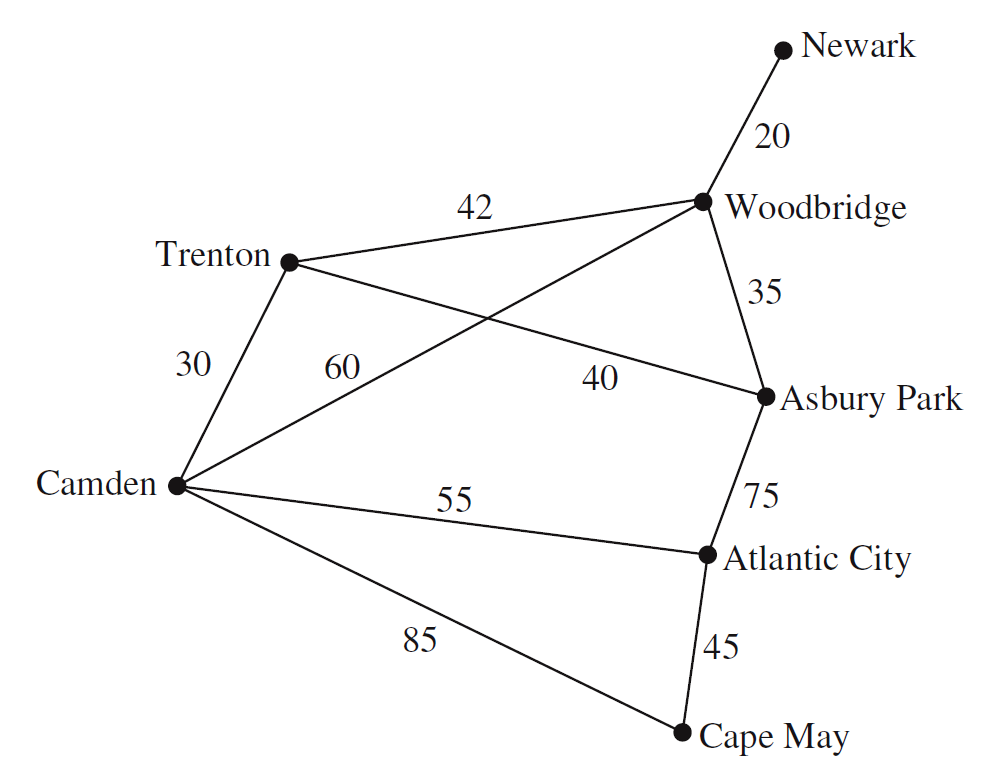
\includegraphics[width=\linewidth]{f-10-6-e-17-a}
			\end{figure}
		\end{column}
	\end{columns}
	\onslide<2>\begin{solution*}
		\begin{description}
			\item[Camden] 80
			\item[Cape May] 165
		\end{description}
	\end{solution*}
\end{frame}

\plain{Questions?}

\end{document}
